
\documentclass{beamer}
\usecolortheme{dove}
\setbeamertemplate{navigation symbols}{}
\usepackage{amsmath,amssymb,amsfonts,amsthm, multicol, subfigure, color}
\usepackage{bm}
\usepackage{graphicx}
\usepackage{tabularx}
\usepackage{booktabs}
\usepackage{hyperref}
\usepackage{pdfpages}
\usepackage{xcolor}
\definecolor{seagreen}{RGB}{46, 139, 87}
\def\independenT#1#2{\mathrel{\rlap{$#1#2$}\mkern2mu{#1#2}}}
\newcommand\indep{\protect\mathpalette{\protect\independenT}{\perp}}
\def\log{\text{log}}
\newcommand\logit{\text{logit}}
\newcommand\iid{\stackrel{\text{iid}}{\sim}}
\newcommand\E{\text{E}}
\newcommand\V{\text{V}}
\renewcommand\P{\text{P}}
\newcommand{\Cov}{\text{Cov}}
\newcommand{\Cor}{\text{Cor}}
\newcommand\doop{\text{do}}
\usepackage{stackrel}
\usepackage{tikz}
\usetikzlibrary{arrows,shapes.arrows,positioning,shapes,patterns,calc}
\newcommand\slideref[1]{\vskip .1cm \tiny \textcolor{gray}{{#1}}}
\newcommand\red[1]{\color{red}#1}
\newcommand\blue[1]{\color{blue}#1}
\newcommand\gray[1]{\color{gray}#1}
\newcommand\seagreen[1]{\color{seagreen}#1}
\newcommand\purple[1]{\color{purple}#1}
\newcommand\orange[1]{\color{orange}#1}
\newcommand\black[1]{\color{black}#1}
\newcommand\white[1]{\color{white}#1}
\newcommand\teal[1]{\color{teal}#1}
\newcommand\magenta[1]{\color{magenta}#1}
\newcommand\Fuchsia[1]{\color{Fuchsia}#1}
\newcommand\BlueGreen[1]{\color{BlueGreen}#1}
\newcommand\bblue[1]{\textcolor{blue}{\textbf{#1}}}
\newcommand\bred[1]{\textcolor{red}{\textbf{#1}}}
\newcommand\bgray[1]{\textcolor{gray}{\textbf{#1}}}
\newcommand\bgreen[1]{\textcolor{seagreen}{\textbf{#1}}}
\newcommand\bref[2]{\href{#1}{\color{blue}{#2}}}
\colorlet{lightgray}{gray!40}
\pgfdeclarelayer{bg}    % declare background layer for tikz
\pgfsetlayers{bg,main} % order layers for tikz
\newcommand\mycite[1]{\begin{scriptsize}\textcolor{darkgray}{(#1)}\end{scriptsize}}
\newcommand{\tcframe}{\frame{
%\small{
\only<1|handout:0>{\tableofcontents}
\only<2|handout:1>{\tableofcontents[currentsubsection]}}
%}
}

\usepackage[round]{natbib}
\bibliographystyle{humannat-mod}
\setbeamertemplate{enumerate items}[default]
\usepackage{mathtools}

\newcommand{\goalsframe}{\begin{frame}{Learning goals for the course}
As a result of participating in this course, students will be able to \vskip .1in
\begin{itemize}
    \item define counterfactuals as the outcomes\\of hypothetical interventions \vskip .1in
    \item identify counterfactuals by causal\\assumptions presented in graphs \vskip .1in
    \item estimate counterfactual outcomes by pairing\\those assumptions with statistical evidence
\end{itemize}
\end{frame}}

\title{Causal Inference: Course Recap}
\author{Cornell STSCI / INFO / ILRST 3900\\Fall 2023\\\bref{https://causal3900.github.io/}{causal3900.github.io}}
\date{30 Nov 2023}

\begin{document}

\maketitle

\goalsframe

\begin{frame}
\includegraphics[width = \textwidth]{figures/mediterranean_diet}
\end{frame}

\begin{frame}{Fundamental problem of causal inference}{\href{https://www.tandfonline.com/doi/abs/10.1080/01621459.1986.10478354}{Holland 1986}}

\begin{tikzpicture}[x = \textwidth, y = .8\textheight]
\node at (0,0) {};
\node at (1,1) {};
% Factual outcomes
\node[anchor = north, align = center] at (.25,1) {Descriptive evidence};
\foreach \i in {1,...,8} {
	\node[font = \tiny, anchor = west] at (-.05,9/20-\i/20 + .175) {Person \i};
}
\foreach \i in {.2,.3,.35,.45,.55} {
	\draw[fill = blue, opacity = .3, color = blue] (.05,\i) rectangle (.25,\i + .05) {};
	\node[font = \tiny] at (.15,\i + .025) {lifespan};
}
\foreach \i in {.25,.4,.5} {
	\draw[fill = seagreen, opacity = .3, color = seagreen] (.25,\i) rectangle (.45,\i + .05) {};
	\node[font = \tiny] at (.35,\i + .025) {lifespan};
}
\node[font = \footnotesize, align = center, fill = blue, fill opacity = .3, text opacity = 1] at (.15,.8) {average\\lifespan};
\node[font = \footnotesize, align = center, fill = seagreen, fill opacity = .3, text opacity = 1] at (.35,.8) {average\\lifespan};
\node at (.25,.8) {$-$};
%\node[font = \tiny] at (.15,.575) {$Y_1^\text{Mediterranean Diet}$};
%\node[font = \tiny] at (.35,.525) {$Y_2^\text{Standard Diet}$};
%\node[font = \tiny] at (.15,.475) {$Y_3^\text{Mediterranean Diet}$};
%\node[font = \tiny] at (.35,.425) {$Y_4^\text{Standard Diet}$};
%\node[font = \tiny] at (.15,.375) {$Y_5^\text{Mediterranean Diet}$};
%\node[font = \tiny] at (.15,.325) {$Y_6^\text{Mediterranean Diet}$};
%\node[font = \tiny] at (.35,.275) {$Y_7^\text{Standard Diet}$};
%\node[font = \tiny] at (.15,.225) {$Y_8^\text{Mediterranean Diet}$};
\node[anchor = north, align = center, font = \footnotesize, blue] at (.15, .2) {Outcome\\under\\Mediterranean\\diet};
\node[anchor = north, align = center, font = \footnotesize, seagreen] at (.35, .2) {Outcome\\under\\standard\\diet};
% Potential outcomes
\node[anchor = north, align = center] at (.75,1) {Causal claim};
\node[font = \footnotesize, align = center, fill = blue, fill opacity = .3, text opacity = 1] at (.65,.8) {average\\lifespan};
\node[font = \footnotesize, align = center, fill = seagreen, fill opacity = .3, text opacity = 1] at (.85,.8) {average\\lifespan};
\node at (.75,.8) {$-$};
\foreach \i in {.2,.25,.3,.35,.4,.45,.5,.55} {
	\draw[fill = blue, opacity = .3, color = blue] (.55,\i) rectangle (.75,\i + .05) {};
	\draw[fill = seagreen, opacity = .3, color = seagreen] (.75,\i) rectangle (.95,\i + .05) {};
	\node[font = \tiny] at (.65,\i + .025) {lifespan};
	\node[font = \tiny] at (.85,\i + .025) {lifespan};
}
\node[anchor = north, align = center, font = \footnotesize, blue] at (.65, .2) {Outcome\\under\\Mediterranean\\diet};
\node[anchor = north, align = center, font = \footnotesize, seagreen] at (.85, .2) {Outcome\\under\\standard\\diet};
\foreach \i in {.2,.3,.35,.45,.55} {
	\node[font = \tiny, red] at (.35,\i + .025) {missing};
}
\foreach \i in {.25,.4,.5} {
	\node[font = \tiny, red] at (.15,\i + .025) {missing};
}
\node at (.5,.66) {Causal inference is a \bred{missing data} problem};
\end{tikzpicture}
\end{frame}

\begin{frame}{Potential outcomes}

\begin{huge}
\centering
$$Y_i^a$$
\end{huge}
the outcome $Y$\\
of person $i$\\
if exposed to treatment $A = a$

\end{frame}

\begin{frame}{Potential outcomes}
\includegraphics[width = \textwidth]{figures/nike_vaporfly}\footnote{Image source: \href{https://www.nike.com/t/zoomx-vaporfly-next-2-mens-road-racing-shoes-glWqfm}{Nike}}
\end{frame}

\begin{frame}{Potential outcomes}

\begin{huge}
\centering
$$Y_i^{a_i,a_j}$$
\end{huge}
the outcome $Y$\\
of person $i$\\
if exposed to treatment $a_i$\\
and their friend exposed to $a_j$

\end{frame}

\begin{frame}{Causal identification by the backdoor criterion}

\begin{figure}
\begin{tikzpicture}[x = \textwidth, y = .8\textheight]
\node (a) at (.5, .45) {$A$};
\node (l) at (.3, .45) {$L$};
\node (y) at (.7, .45) {$Y$};
\draw[->, thick] (a) -- (y);
\draw[->, thick, red] (l) to[out = 45, in = 135] (y);
\draw[->, thick, red] (l) -- (a);
\end{tikzpicture}
\end{figure}
{\color{red} Backdoor path} starts with an edge pointing in to $A$ and ends at $Y$


\vspace{1em}
A set of variables satisfies the backdoor criterion if
\begin{enumerate}
     \item Blocks all backdoor paths
     \item Does not contain any descendant of $A$
\end{enumerate}

\vspace{1em}ß
Sufficient adjustment sets satisfy the backdoor criterion!
\end{frame}

\begin{frame}{Estimation}

If conditional exchangeability holds given $\vec{L}$,\\
then we need an estimator that statistically adjusts for $\vec{L}$ \vskip .2in
\begin{itemize}
\item regression
\item inverse probability weighting
\item matching
\end{itemize}

\end{frame}

\begin{frame}{Identification without exchangeability}
\begin{tikzpicture}[x = \textwidth, y = .8\textheight]
\node at (0,0) {};
\node at (1,1) {};
\node[anchor = north west] at (0,.9) {Front Door};
\node (a) at (.05,.67) {$A$};
\node (m) at (.2,.67) {$M$};
\node[red] (u) at (.2,.8) {$U$};
\node (y) at (.35,.67) {$Y$};
\draw[->, thick] (a) -- (m);
\draw[->, thick] (m) -- (y);
\draw[->, thick, red, dashed] (u) -- (a);
\draw[->, thick, red, dashed] (u) -- (y);
\node[anchor = north west] at (.5,.9) {Instrumental Variables};
\node (z) at (.55,.67) {$Z$};
\node (a) at (.7,.67) {$A$};
\node[red] (u) at (.7,.8) {$U$};
\node (y) at (.85,.67) {$Y$};
\draw[->, thick] (z) -- (a);
\draw[->, thick] (a) -- (y);
\draw[->, thick, red, dashed] (u) -- (a);
\draw[->, thick, red, dashed] (u) -- (y);
\node[anchor = south west, align = left] (rd) at (0,.4) {Regression\\Discontinuity};
\node[anchor = north] at (rd.south) {\includegraphics[width = .3\textwidth]{figures/rdd}};
\node[anchor = south west, align = center] (did) at (.33,.4) {Difference in\\Difference};
\node[anchor = north] at (did.south) {\includegraphics[width = .3\textwidth]{figures/did_from_hw}};
\node[anchor = south west, align = center] (synth) at (.66,.4) {Synthetic\\Control};
\node[anchor = north] at (synth.south) {\includegraphics[width = .3\textwidth]{figures/adh_synth}};
\end{tikzpicture}
\end{frame}

\begin{frame}{Course structure}

\begin{itemize}
\item concepts introduced in lecture
\item hands-on practice in discussion
\item reinforced with problem sets
\item project to independently apply what you learned
\end{itemize} \vskip .2in

\includegraphics[width = \textwidth]{figures/website_p1}


\end{frame}

\begin{frame}{Your thoughts}
\begin{itemize}
\item What could we do to make this course better?
\item What is your favorite thing you learned?
\item What parts do you anticipate being most useful for your future work?
\end{itemize}
\end{frame}

\begin{frame}{Evaluations}

We want to hear from you! \vskip .3in

We encourage \bblue{specific examples} for your TAs \vskip .05in

\begin{itemize}
\item Recitation or discussion
\begin{itemize}
\item Comments on the recitation or discussion section (include day and time of section or TA name)
\end{itemize}
\item Comparison to other courses
\begin{itemize}
\item If you would like to nominate a TA from this course for a teaching award, please identify
the TA and explain briefly why.
\end{itemize}
\end{itemize}

\end{frame}

\begin{frame}{Drop us a line!}
\Large

In the future, if you are using any of the material from class, we'd love to know! 
\end{frame}


\goalsframe

\end{document}

